\documentclass[12pt,a4paper]{article}
\usepackage[utf8x]{inputenc}
\usepackage{ucs}
\usepackage[spanish]{babel}
\usepackage{amsmath}
\usepackage{amsfonts}
\usepackage{amssymb}
\usepackage{makeidx}
\usepackage{graphicx}
\usepackage[width=17.00cm, height=23.00cm]{geometry}
\usepackage{hyperref}
\author{
	C411-Dalianys Pérez Perera\\C411-Dayany Alfaro González\\C411-Gilberto González Rodríguez
}
\date{}
\title{Mini proyecto de Clase Práctica 7 de Estadísticas}
\begin{document}
	\maketitle
	\section{Ejercicio 1}
	\textbf{a-)} Las variables independientes son el Mes y el Gasto, la variable dependiente las Ventas. El Mes está claro que es independiente. Con respecto al gasto y las ventas tiene más sentido que las ventas dependan del gasto puesto que, considerando que los gastos se realizan para aumentar la producción o para invertir en la calidad de los productos, las ventas de la empresa van a aumentar.
	
	\textbf{b-)} El modelo se realiza con la variable Gasto. El coeficiente de correlación entre Gasto y Ventas es 0.9988322 lo que implica que hay una relación líneal fuerte. Por lo tanto tiene sentido hacer la regresión lineal.\\
	Además el modelo de dispersión muesta la correlación lineal de ambas variables.\\
	\begin{figure}[h!]
		\centering
		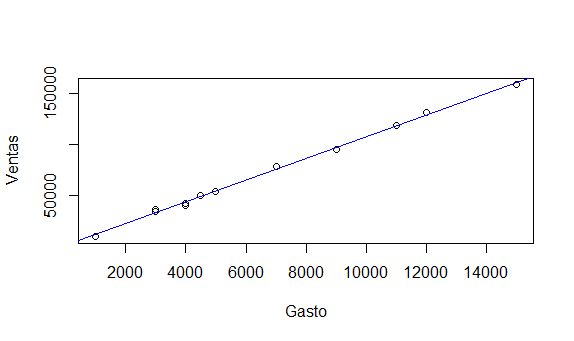
\includegraphics[scale=0.8]{GxV.png}
	\end{figure}
	
	\newpage
	
	El summary de la regresión lineal en R es:\\
	
	Residuals:\\

	\begin{tabular}{ccccc}
		Min&     1Q& Median&     3Q&    Max\\
		-3385&  -2097&    258&   1726&   3034 
	\end{tabular}\\ 
	
	Coefficients:\\

	\begin{tabular}{cccccc}
		 &     Estimate & Std. Error&     t value&   $Pr(>|t|)$&\\
		(Intercept) & 1383.4714 & 1255.2404 &  1.102  &  0.296&\\
		 Gasto      &   10.6222 &   0.1625  & 65.378  & 1.71e-14 &***\\
	\end{tabular}\\
	
	Signif. codes:  0 ‘***’ 0.001 ‘**’ 0.01 ‘*’ 0.05 ‘.’ 0.1 ‘ ’ 1\\
	
	Residual standard error: 2313 on 10 degrees of freedom\\
	
	Multiple R-squared:  0.9977,	Adjusted R-squared:  0.9974\\ 
	
	F-statistic:  4274 on 1 and 10 DF,  p-value: 1.707e-14\\
	
	
	De la columna Estimate en Coefficients se puede extraer que $\beta_0=1383.4714$ y $\beta_1=10.6222$, por lo que el modelo que4todaría como:
	\begin{equation*}
	{Ventas}^{*} = 1383.4714 + Gasto * 10.6222
	\end{equation*}
	
	Sobre los coeficientes se puede decir que el intercepto es mucho mayor que el coeficiente de la variable independiente, esto quiere decir que hay gran parte de las Ventas de la población que no están explicadas a aprtir del Gasto, se pudieran hacer dos cosas, adicionar más variables al modelo, lo que se hará en el siguiente inciso, y en caso de no contar con más variables se puede realizar una transformación lineal y aplicar la regresón a las variables transformadas para obtener un valor más pequeño del intercepto. 
	El coeficiente del gasto es significativo al $0\%$, ya que su $Pr(>|t|)$ para es $1.71e-14$, mucho menor que $0.05$, casi cero, mientras que el intercepto es significativo al $30\%$, lo cual es muy malo. Los coeficientes también indican que por cada unidad de incremento del Gasto se espera que las Ventas aumenten en $10.6$ unidades.\\
	
	Como el $Pr(>|t|)$ del gasto es menor que $0.05$ entonces el coeficiente sí está aportando al modelo, sin embargo el valor de $Pr(>|t|)$ para el intercepto es $0.296$, lo que implica que este no está aportando nada significativo al modelo.\\
	
	A pesar de que que R-cuadraro tiene más sentido analizarlo en un modelo de regresón múltiple, este valor cuanto más cercano a 1 mejor, en este caso es $0.997$, lo cual es bueno. El error estandar nos permite compara este modelo con otros que tengan similare valore de R-cuadrado ajustado.\\ 
	
	Sin embargo dado que el p-valor de la prueba F, es menor que $0.05$ se puede concluir que al menos una variable es significativamente diferente de cero en el modelo.\\
	
	\textbf{Analizando los supuestos:}\\
	
	\textbf{1-) La media de los errores es cero y la suma de los errores es cero.}\\
	 
	La media de los residuales es $-2.368846e-13$ y la suma $-2.842171e-12$ por lo que se puede decir que sí se cumple el supueto, ambos valores son bien cercanos a cero.\\
	
	\textbf{2-) Errores normalmente distribuidos.} \\
	
	\begin{figure}[h!]
		\centering
		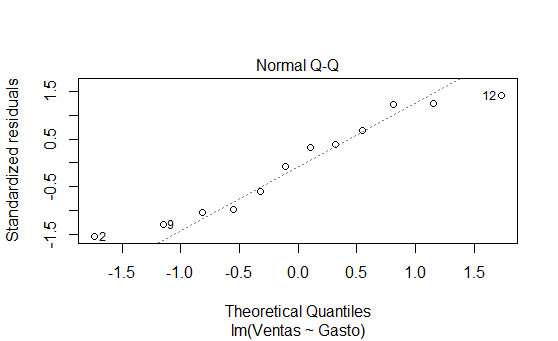
\includegraphics[scale=0.8]{simplemodel_qqplot.png}
	\end{figure}
	
	Como solo se ven unos cuantos puntos aislados y la mayoría están cerca de la recta se puede asumir la normalidad de los datos.\\ 
	
	\textbf{3-) Independencia de los residuos.}\\
	data:  modelo lineal\\
	$DW = 1.1347$, $p-value = 0.03062$\\
	alternative hypothesis: true autocorrelation is greater than 0\\
	
	Como el p-valor es $0.03062$ menor que $0.05$, se puede rechazar la hipótesis nula por lo tanto los residuos no son independientes y el modelo no cumple este supuesto.\\
	
	\newpage
	
	\textbf{4-) Homocedasticidad.}\\
	
	\begin{figure}[h!]
		\centering
		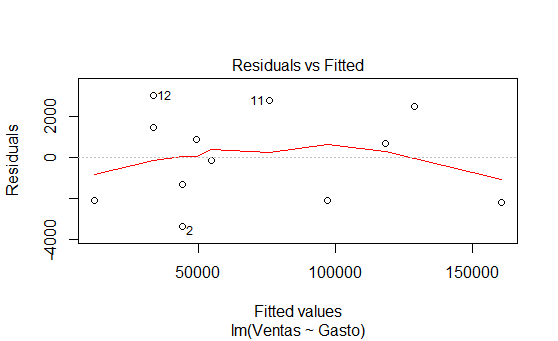
\includegraphics[scale=0.8]{simpleResidualasVsFitted.png}
	\end{figure}

	\textbf{c-)} Regresión lineal múltiple
	
	\section{Ejercicio 3} 
		
\end{document}